\documentclass{standalone}
\usepackage{tikz}

\begin{document}
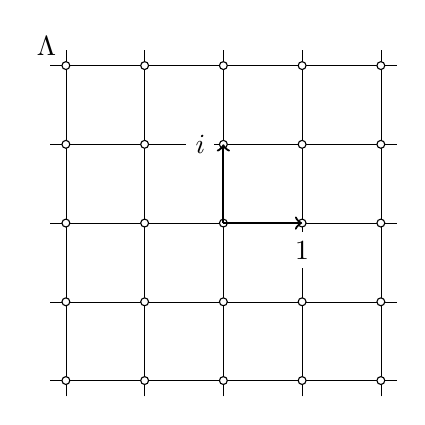
\begin{tikzpicture}
\foreach \h in {-2,-1,...,2}{
  \draw[ultra thin] (-2.2,\h) -- (2.2,\h);
  \draw[ultra thin] (\h,-2.2) -- (\h,2.2);
}
\foreach \x in {-2,-1,...,2} {
	\foreach \y in {-2,-1,...,2} {
    \filldraw[fill=white] (\x, \y) circle[radius=0.05];
	};
};
\draw[thick, ->] (0,0) -- (0,1) node[left=0.1cm, fill=white]{$ i $};
\draw[thick, ->] (0,0) -- (1,0) node[below=0.1cm, fill=white]{$ 1 $};
\draw (-2,2) node[anchor=south east]{$ \Lambda $};
\end{tikzpicture}
\end{document}

